\section{Experiments}
\subsection{Simulation Setup}
\begin{figure}[h]
	\centering
	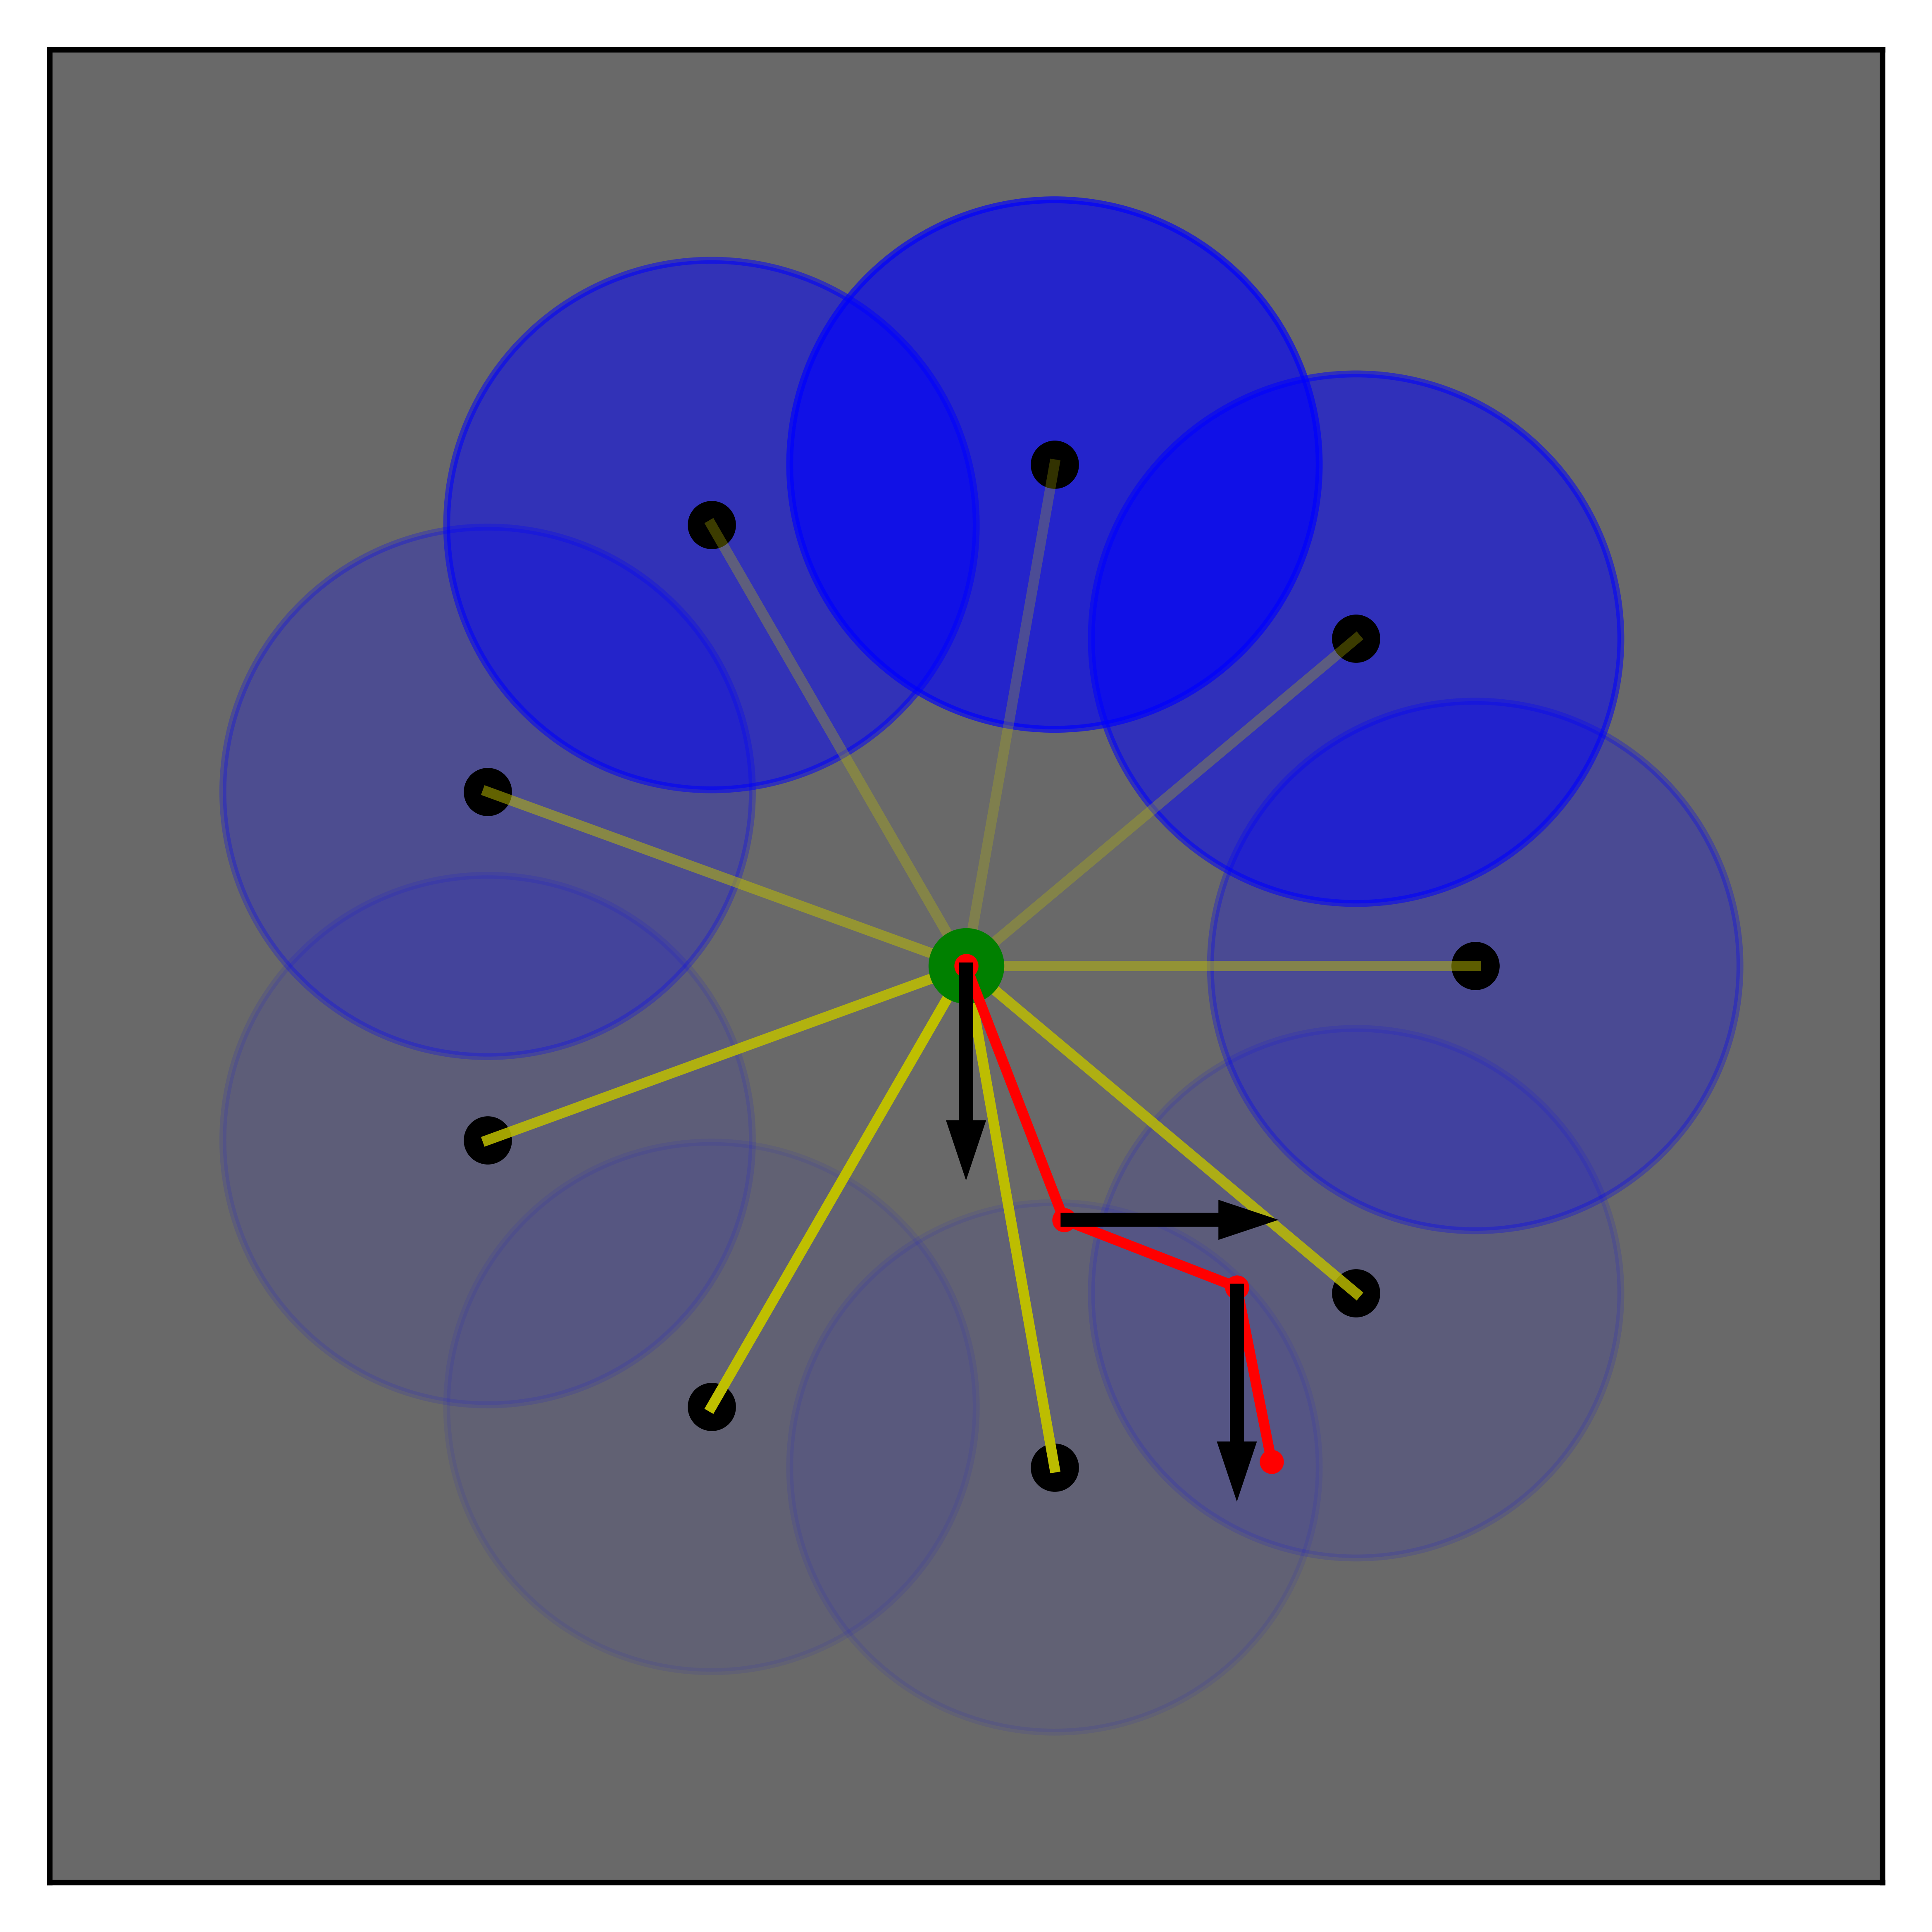
\includegraphics[width= 0.4\linewidth,clip]{actions}
	\caption{The agent path as dictated by the optimal actions, overlayed with the actions selected by the maximum lower bound on the Q-function for $\kappa=0.5$. In this case the maximum lower bound was in agreement with the optimal action, this is not always the case. The beacon intensity denotes its probability of success. And the line intensities are directly proportional to the covariance of the observation factor used as an initial belief.}
	\label{fig:actions}
\end{figure}
As discussed in \cref{sec:complete_elimination}, \cref{thm:bounds_elim} can be utilized alongside \eqref{eq:remove_da} when formulated for expected reward. The following simulations demonstrate the improvement in runtime and the resulting bounds obtained upon utilizing the aforementioned inequalities.

We consider planning in the landmark-SLAM scenario, a high-dimensional smoothing problem where the state space expands over time to include current and past poses, as well as landmarks in $\mathbb{R}^2$. The action space consists of unit circle motion primitives. The transition model is given by $\state{}^\prime=\state{}+\action{}+\omega_{\action{}}$ where $\omega_{\action{}}\sim N(0,\Sigma_{\action{}})$, and the observation model is given by $\observation{}{}=\landmark{}-\state{}+\omega_{\observation{}{}}$, where $\omega_{\observation{}{}}\sim N_r(0,\Sigma_{\observation{}{}})$.  $N(0,\Sigma_\action{})$ is a multivariate zero-mean Gaussian distribution with covariance $\Sigma_{\action{}}$ and $N_r(0,\Sigma_{\observation{}{}})$ is a multivariate zero-mean Gaussian distribution with covariance $\Sigma_{\observation{}{}}$ truncated at radius $r$, allowing for an infimum greater than zero, which is reasonable given noise filtering and outlier pruning practices. Observations are relative position between poses and landmarks. Each landmark $\landmark{i}$ has probability $p_i$ to succeed in sending an observation to the agent once the agent is within a radius $r$ of the landmark (i.e. $\probcond{\da{}{i}}{\state{},\landmark{i}}=\1{\norm{\state{}-\landmark{i}}\leq r}p_i$). The reward is given to be negative entropy as the task is information gain.

An initial belief over the agent pose and landmarks is instantiated via a prior on the initial pose and observation factors to each landmark. Subsequently belief tree is constructed using sparse sampling, where, in addition to action and observation nodes, we introduce DA nodes (see \cref{fig:topology}). High-dimensional inference is handled incrementally using the slices approach from~\cite{Shienman24arxiv}. After constructing the tree in a downward pass, rewards, expected reward bounds, and Q-functions are calculated in an upward pass while maintaining Bellman optimality. In the case of bounds on the Q-function, the maximum over the lower and upper bounds are passed up. We define $\kappa$ as $\frac{\abs{\subSpace}}{\abs{\mathcal{D}}}$, representing the proportion of DA nodes eliminated for the expected reward bounds.  When $\kappa=1$ no nodes are eliminated and the expected reward remains unchanged; for $\kappa=0$ all $\da{}{}$ realizations are discarded, resulting in loose bounds on the expected reward. Specifically, $\kappa$ splits $\mathcal{D}$ into two sets: $\da{}{}\in\subSpace$ and $\tilde{\da{}{}}\in\stcomp{\subSpace}$ as required for \cref{thm:bounds_elim}. The reference DA, $\da{}{}$, is used to calculate bounds on $\condEntropy{\statesRV{}}{\observationsRV{},\tilde{\da{}{}}}$; the selection process of a reference DA is not addressed in this work, and we simply select a reference DA such that $\da{\textup{diff}}{}\neq0$. Joint state sampling via~\cite{Shienman24arxiv} allows access to the estimated joint likelihood which was used to evaluate the reward. The weighted samples represent our belief over the state for reward calculations, using the same samples for both rewards and bounds.

\subsection{Results}
\begin{figure}[h]
	\centering
	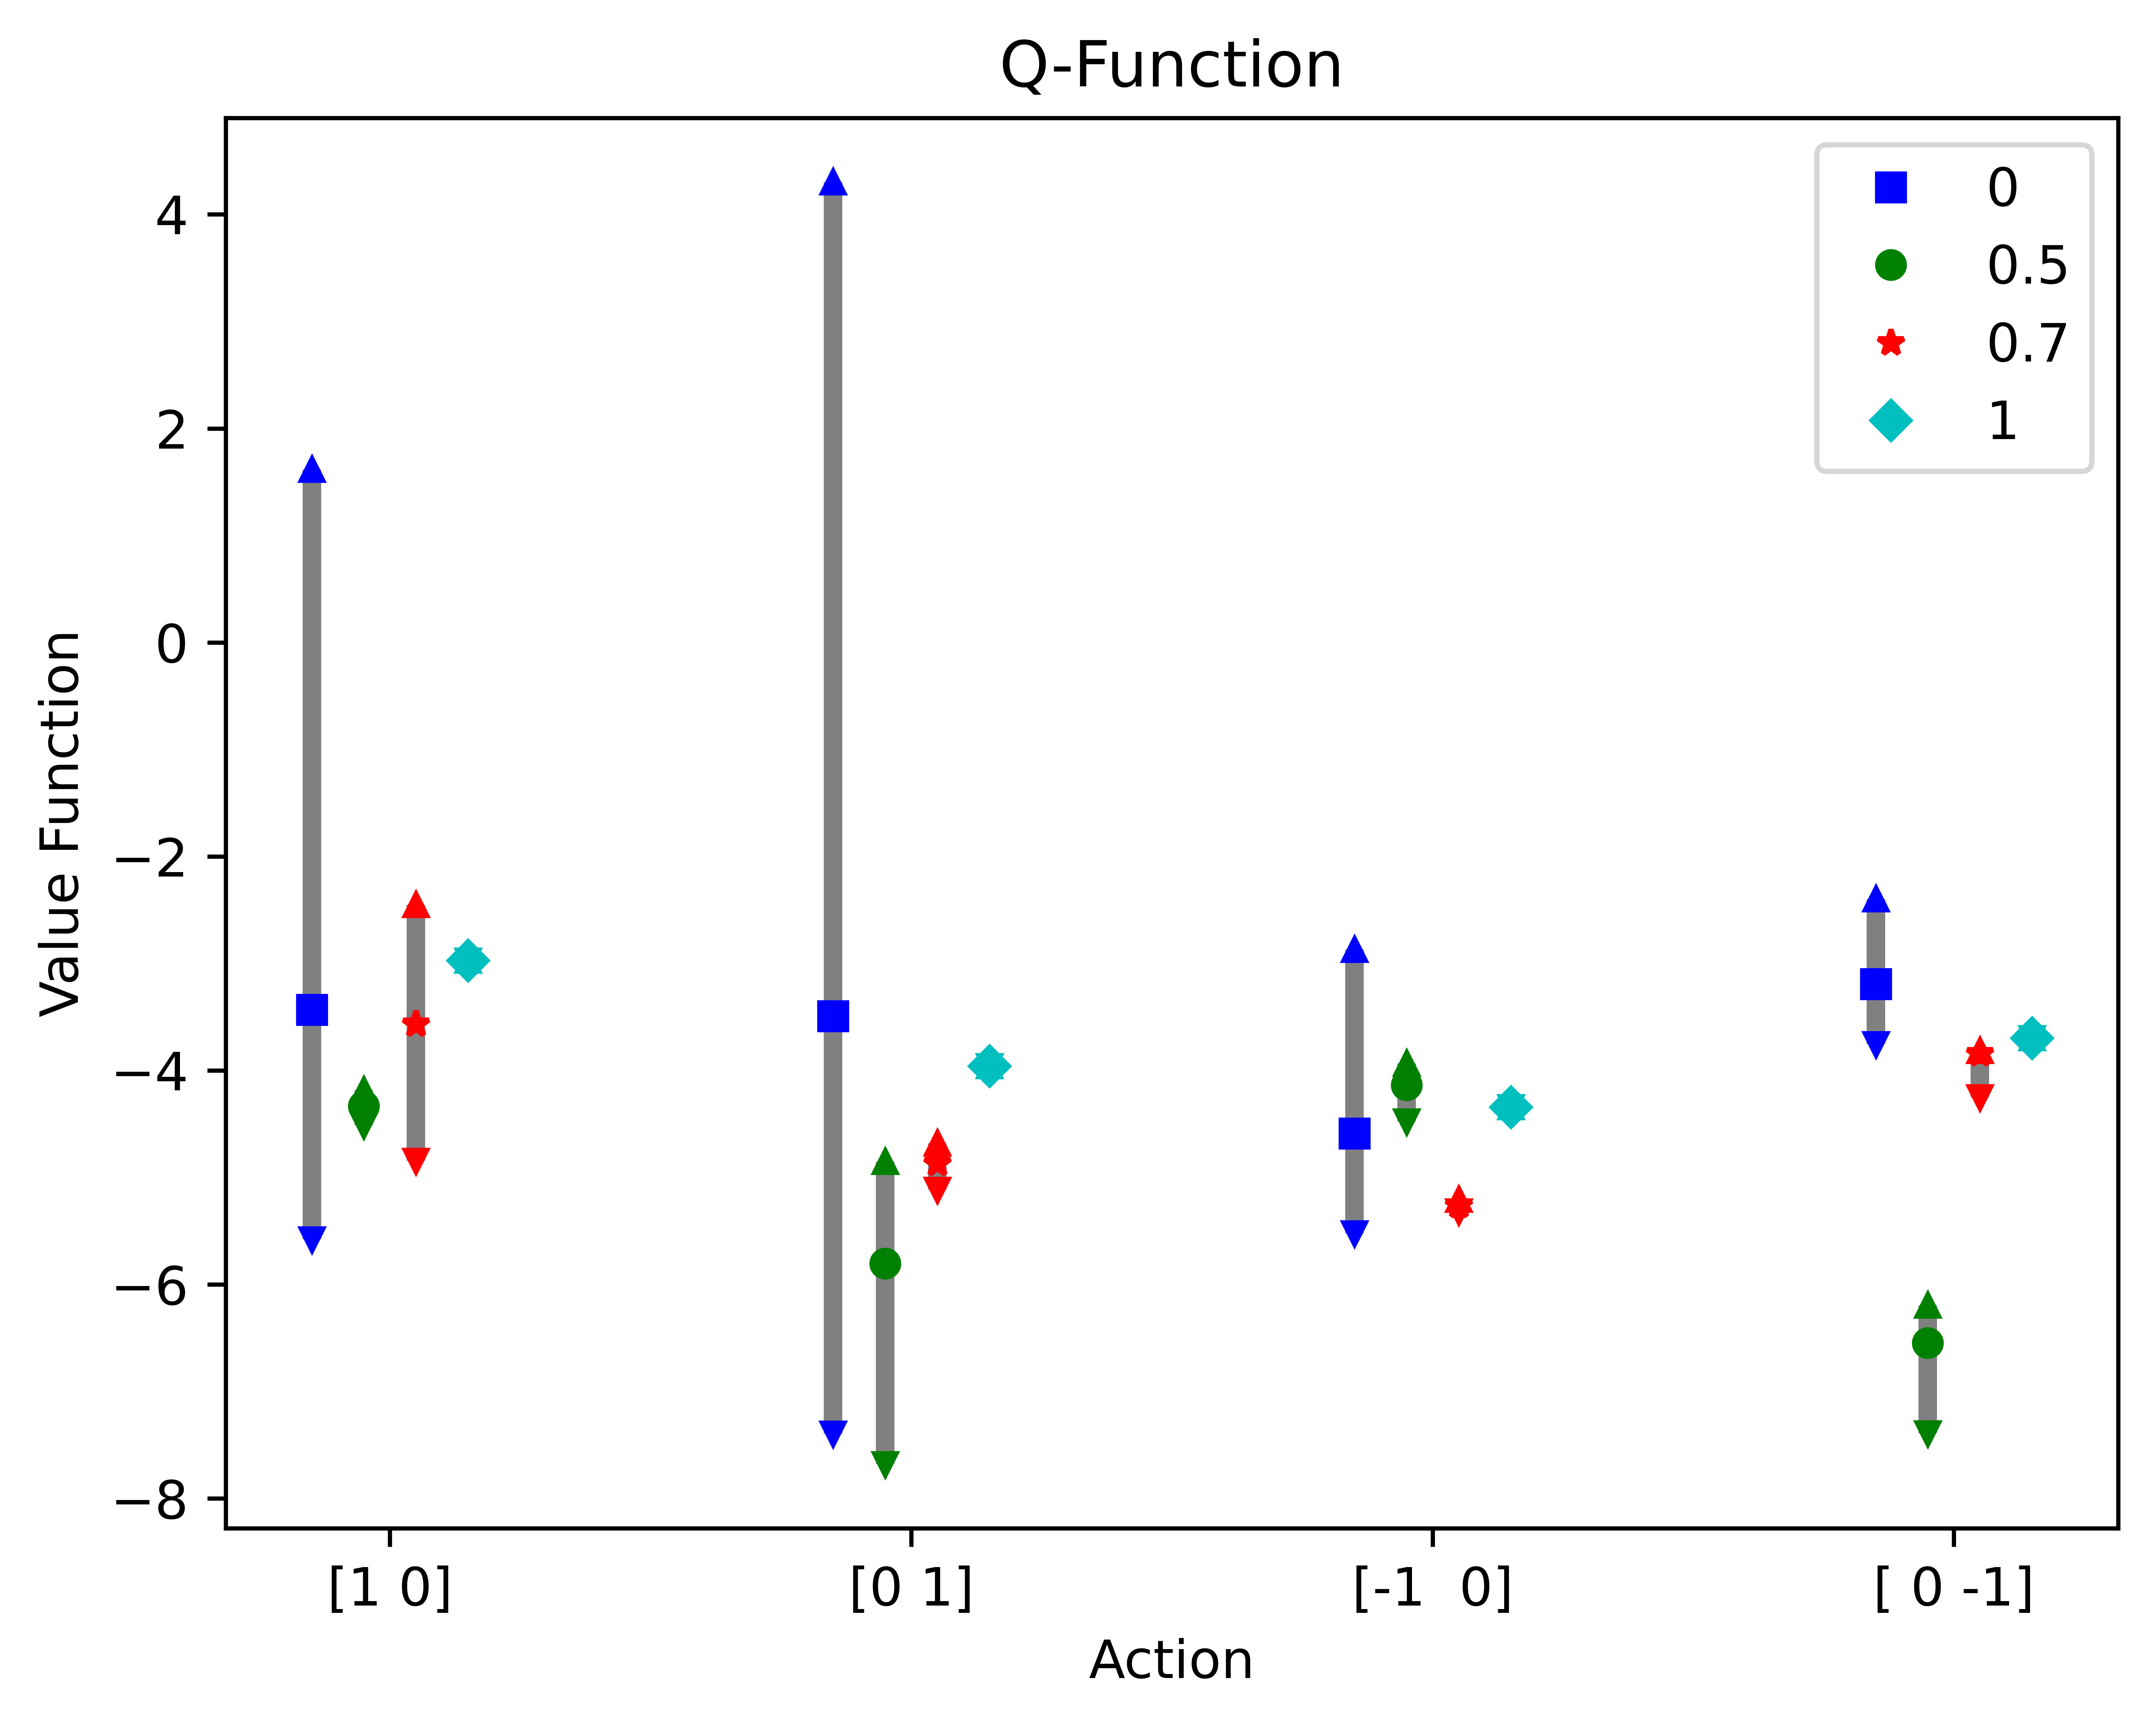
\includegraphics[width= 0.4\linewidth,clip]{q_function}
	\caption{Comparison\tablefootnote{Source code: \url{https://github.com/ohadlor/bounded_POMDP_planner}} of the Q-functions alongside the bounds calculated on the Q-functions for various values of $\kappa$.}
	\label{fig:q_function}
\end{figure}
From \cref{fig:q_function} we first note that for $\kappa=0$ the bounds are most loose, but offer a significant speedup as shown if \cref{table:results}. In essence, these are the free bounds. For $\kappa=1$ we find that the bounds converge to the optimal Q-function and no penalty is suffered to the speedup. Finally for $\kappa=\numlist{0.5;0.7}$ we observe a speedup of $\times$\numlist{2.6;1.3} respectively. Although the bounds on the Q-function overlap in both cases, not permitting optimal action selection, they do allow for action elimination. For $\kappa=0.7$ actions \numlist{2;3} can be eliminated, for $\kappa=0.5$ actions \numlist{2;4} can be eliminated. The Q-function bounds for a given $\kappa$ differ in looseness as the bounds are proportional to $\measure{\stcomp{\subSpace}}$ and so depend on the DA eliminated. As higher weighted DA nodes are discarded, the bounds are proportionally weighted, the benefit being that often times DA nodes with higher likelihood must be traversed more times for evaluating the reward. Finally, as the number of DA nodes per action is limited in our simulation, often times we must take $\da{\textup{ref}}{}=0$, as for all other $\da{\textup{ref}}{}$ $\da{\textup{diff}}{}=0$. Finally, due to the discrete nature of the division of $\mathcal{D}$, as $\abs{\mathcal{D}}$ grows, the value of $\frac{\abs{\subSpace}}{\abs{\mathcal{D}}}$ approaches the pre-defined $\kappa$.
\begin{table}
	\centering
	\caption{A value of $q=2$ was selected for \cref{thm:bounds_elim}. 150 samples were used for inference, 150 observations per action for sparse sampling, and 100 samples for reward calculations.}\label{table:results}
	\scalebox{0.8}{
	\begin{tabular}{|c|c|c|c|c|}
		\hline
		$\kappa$\tablefootnote{results are averaged over three runs.}&  No. Eliminated Factors & Reward Runtime [\unit{\second}] & Bounds Runtime [\unit{\second}] & Speedup \\
		\hline
		\num{1} & \num{0\pm 0} & \num{876.5 \pm164.5} & \num{874.0\pm 164.5} & \num{1.0\pm0.0} \\
		\hline
		\num{0.7} & \num{88\pm 45} & \num{991.1 \pm446.6} & \num{743.7\pm 283.4} & \num{1.3\pm0.1} \\
		\hline
		\num{0.5} & \num{189\pm 92} & \num{720.8 \pm43.0} & \num{295.0\pm 94.5} & \num{2.6\pm0.4} \\
		\hline
		\num{0} & \num{330\pm 164} & \num{651.7\pm123.5} & \num{16.3\pm 0.6} & \num{39.8\pm7.1} \\
		\hline
	\end{tabular}}
\end{table}

